\documentclass[conference]{IEEEtran}
\usepackage{graphicx}
\usepackage{booktabs}
\usepackage{amsmath,amssymb}
\usepackage{url}
\usepackage{xcolor}
\usepackage[hidelinks]{hyperref}
\graphicspath{{../results/figures/}}

\begin{document}

\title{Indoor Location Prediction from Wi-Fi Signal Strength:\\ A Machine Learning Baseline on UJIIndoorLoc}

\author{
\IEEEauthorblockN{Rishi Raj (2401010380), Aditya Samadhiya (2401010037), Yash Yadav (2401010515),\\ Kaustubh Ranjan Mishra (2401020116), Yash Raj (2401010514)}
\IEEEauthorblockA{Advanced Machine Learning --- Project 9, Phase 1\\
Section D, Rishihood University}
}

\maketitle

\begin{abstract}
GPS does not work reliably indoors, but almost every building is covered by Wi-Fi. We predict a
phone's building, floor and $(x,y)$ position from a single scan of Wi-Fi received signal strengths
(RSSI), using the public UJIIndoorLoc dataset (3 buildings, 13 building--floor classes, 520 access
points, 21{,}048 scans). The data is extremely sparse: 96.5\% of the readings are ``not detected''.
We clean the data, handle the missing-signal convention consistently, and compare
linear/logistic regression, $k$-nearest neighbours and Random Forests, including a hierarchical
Random Forest that first predicts the building and then uses a per-building model. All choices are made by
5-fold cross-validation grouped by user, and the official validation file, collected four months
later, is used only once as the test set. On the test set, the per-building Random Forest reaches 99.8\% building accuracy, 91.3\% floor accuracy and 9.37\,m
mean position error (7.07\,m median). $k$-NN achieves the lowest mean error, 8.69\,m, and linear regression fails at
positioning (52\,m), which shows that the signal-to-position mapping is strongly non-linear.
We analyse the errors by building/floor correctness, by phone and by signal coverage, and identify the
gap that Phase~2 (multitask deep learning) will address.
\end{abstract}

\begin{IEEEkeywords}
indoor positioning, Wi-Fi fingerprinting, RSSI, random forest, k-nearest neighbours, UJIIndoorLoc
\end{IEEEkeywords}

\section{Introduction}
Satellite positioning fails inside buildings because walls and roofs block and reflect the signal.
Indoor location is still useful for navigation in campuses and hospitals, for emergency response and for asset
tracking. Wi-Fi access points (APs) are already everywhere, and a phone can measure the RSSI of every AP it
hears without connecting to it. Converting RSSI to distance with a propagation model is unreliable
indoors because of walls, people and multipath reflections~\cite{zafari2019survey}. \emph{Fingerprinting}
avoids modelling propagation: a radio map of RSSI vectors is recorded at known positions, and a new scan is
located by learning from that map~\cite{bahl2000radar}.

The task combines two \textbf{classification} problems (building, floor) and one \textbf{regression}
problem ($x,y$ in metres). Phase~1 of this project builds and validates the machine learning
baseline. Our contributions are:
\begin{itemize}
\item a careful data audit (duplicates, empty scans, a faulty phone, train/test shift);
\item a leakage-free pipeline in which every statistic is fitted on training data, and model
selection uses cross-validation that holds out whole users;
\item a comparison of linear/logistic regression, $k$-NN and Random Forests (plain and hierarchical) on
building accuracy, floor accuracy, coordinate error and the IPIN competition score;
\item a hierarchical error breakdown, floor confusion matrices, coordinate error maps and a per-phone
robustness analysis.
\end{itemize}

\section{Literature Review}
\textbf{Fingerprinting.} RADAR~\cite{bahl2000radar} introduced Wi-Fi fingerprinting with nearest-neighbour
matching in signal space. Horus~\cite{youssef2005horus} modelled the RSSI distribution at each location
probabilistically, which showed how noisy single readings are.

\textbf{UJIIndoorLoc.} Torres-Sospedra \emph{et al.}~\cite{torres2014uji} released our dataset, the first
large multi-building, multi-floor public benchmark, with a $k$-NN baseline reaching 89.9\% floor accuracy
and 7.9\,m mean error. A follow-up study~\cite{torres2015distance} compared 51 distance measures and four data
representations for $k$-NN and found that the \emph{powed} representation, which compresses weak readings,
helps. The IPIN 2016 competition~\cite{torres2017ipin} defined the combined score we report.

\textbf{Machine learning models.} Bozkurt \emph{et al.}~\cite{bozkurt2015comparative} compared decision trees,
naive Bayes, $k$-NN and ensembles on UJIIndoorLoc and found $k$-NN and tree ensembles strongest.
HybLoc~\cite{akram2018hybloc} splits the radio map into clusters and trains a Random Forest~\cite{breiman2001rf}
per cluster, the same divide-and-conquer idea as our per-building model.

\textbf{Deep learning (Phase 2 context).} Stacked autoencoders with an MLP~\cite{nowicki2017lowEffort,kim2018scalable}
and CNNs~\cite{song2019cnnloc} reach about 92--96\% floor accuracy on UJIIndoorLoc. Multitask
learning~\cite{caruana1997mtl}, where related tasks share one representation, motivates our Phase~2 model.

\textbf{Gaps addressed here.} (i) The ``+100 = not detected'' value is often fed to models as a number,
which inverts its meaning. (ii) Random train/validation splits leak near-duplicate scans and overstate accuracy.
(iii) Most baselines model building, floor and position independently.

\section{Dataset and Exploratory Analysis}
\label{sec:eda}
UJIIndoorLoc~\cite{torres2014uji} was collected on the Universitat Jaume~I campus: three buildings with four, four and five floors. Each scan contains 520 RSSI values (dBm; $+100$ means not detected) plus longitude and latitude in metres (UTM),
floor, building, space ID, user ID, phone ID and a timestamp. The training file has 19{,}937 scans from 18 users
and 16 phones (May--June 2013). The validation file has 1{,}111 scans collected four months later (Sept--Oct 2013) by
different users, on 11 phones, 9 of which do not appear in training.

\textbf{Cleaning.} We removed 637 exact duplicate rows and 73 scans in which no AP was heard, leaving 19{,}227 training scans.
The test file is left untouched so that our results stay comparable with the literature.

\begin{figure}[t]
\centering
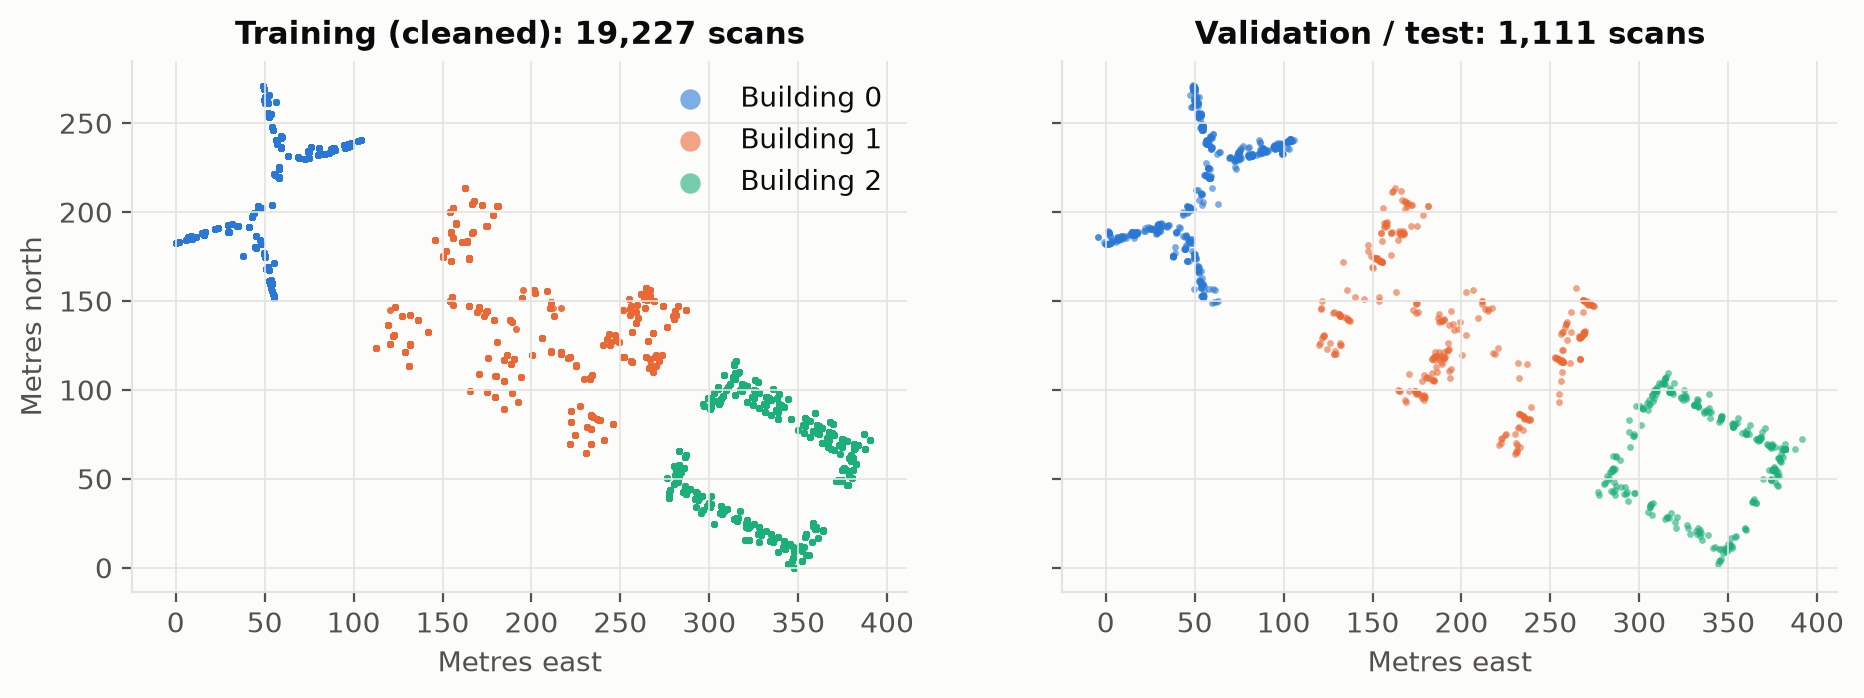
\includegraphics[width=\columnwidth]{eda_campus_map}
\caption{Scan positions. The test set covers the same buildings but is skewed towards building 0.}
\label{fig:map}
\end{figure}

\textbf{Sparsity.} A scan hears about 18 of the 520 APs on average, so 96.5\% of the matrix is ``not
detected'' (Fig.~\ref{fig:sparsity}). Detected RSSI ranges from $-104$ to $0$\,dBm, and most readings are weaker than $-70$\,dBm.
55 APs are never heard in training, and 323 of the remaining 465 are heard in only one building
(Fig.~\ref{fig:locality}). This is why building classification is easy.

\begin{figure}[t]
\centering
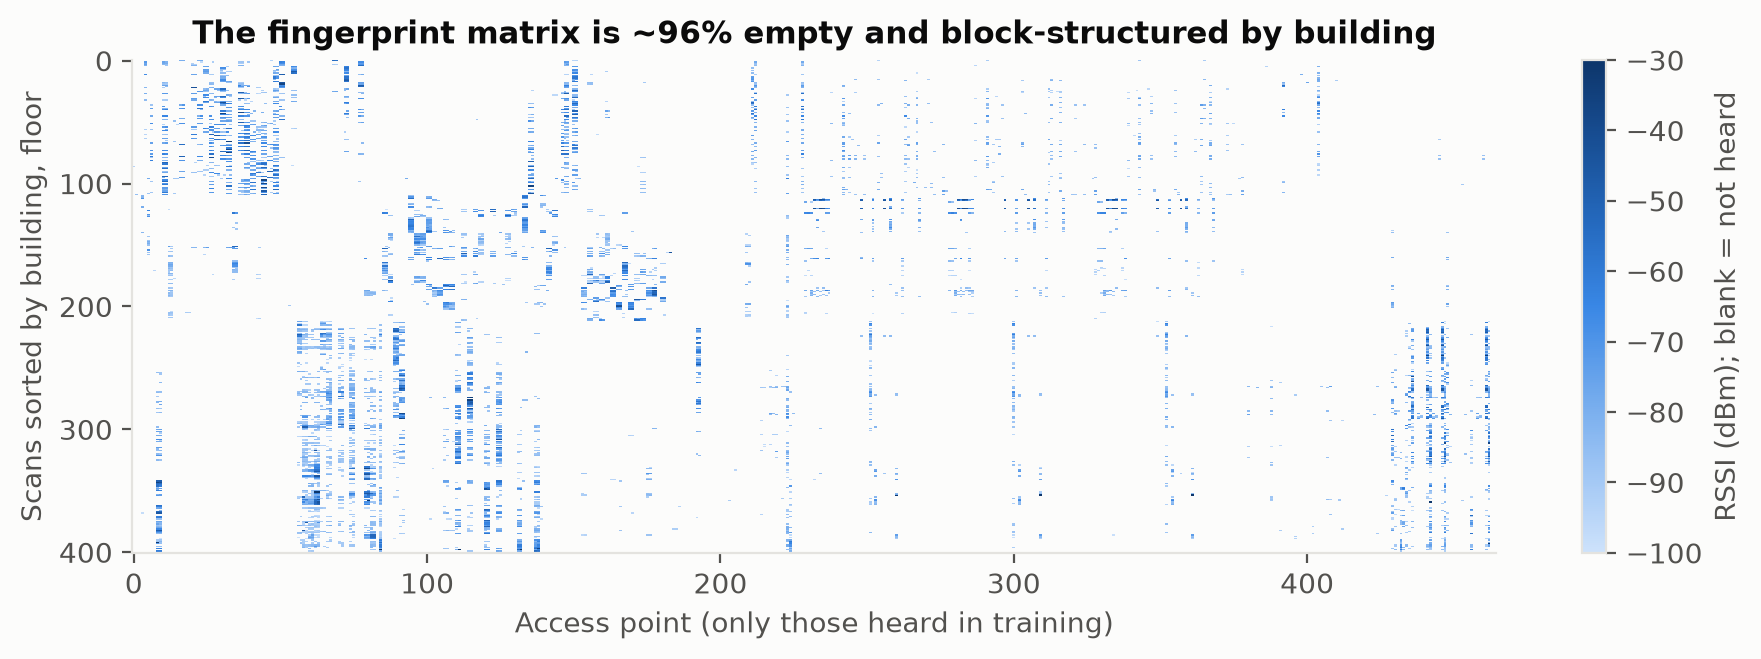
\includegraphics[width=\columnwidth]{eda_sparsity_heatmap}
\caption{Sample of the fingerprint matrix (rows sorted by building and floor). It is about 96\% empty, with block structure per building.}
\label{fig:sparsity}
\end{figure}

\begin{figure}[t]
\centering
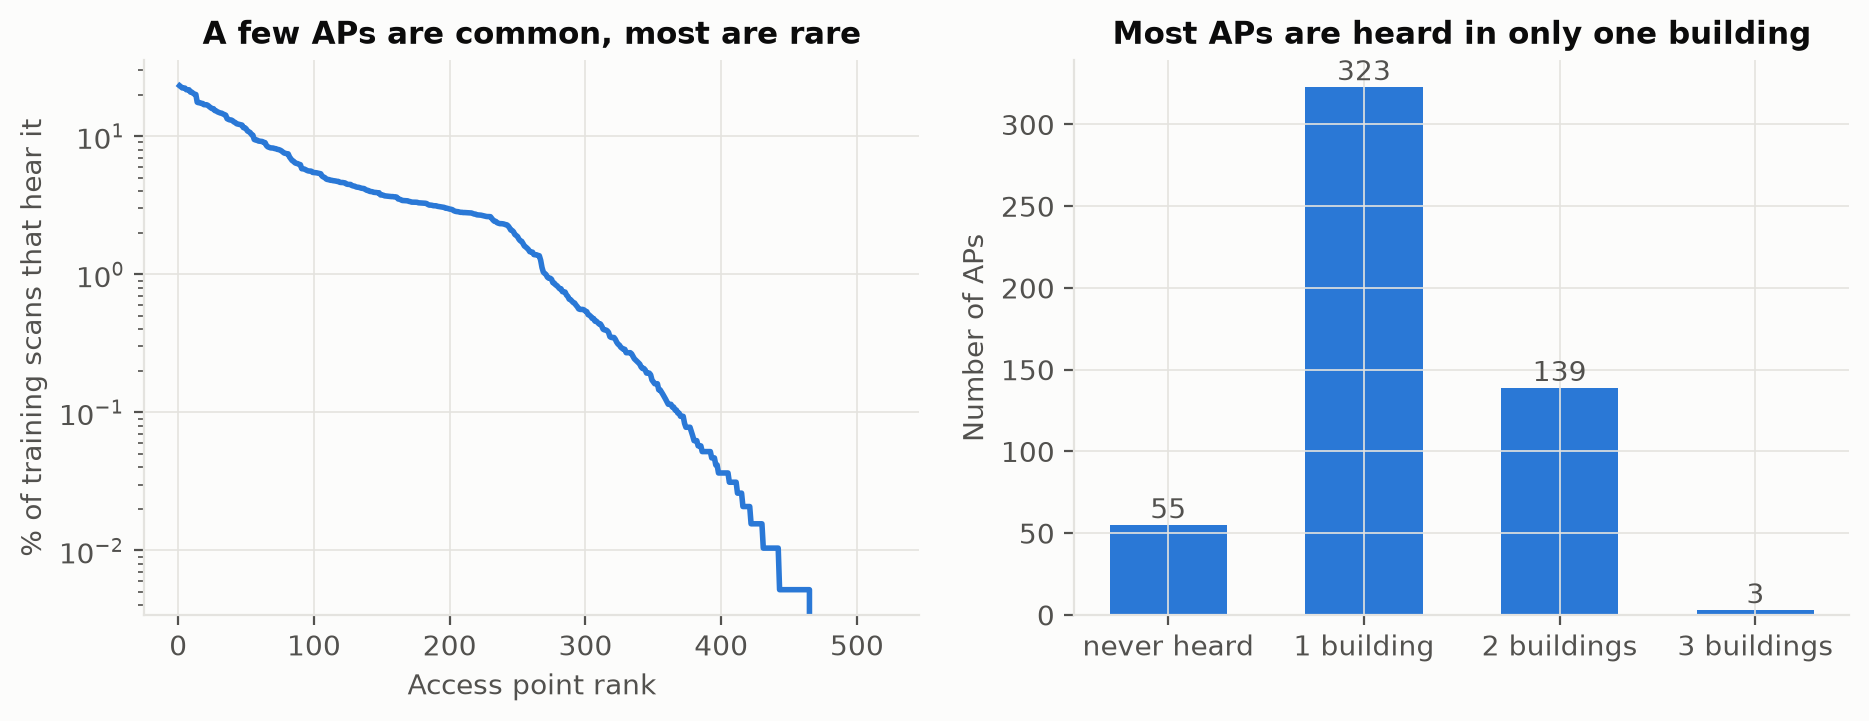
\includegraphics[width=\columnwidth]{eda_ap_locality}
\caption{Left: a few APs are heard often, most rarely. Right: most APs are heard in a single building.}
\label{fig:locality}
\end{figure}

\textbf{Floors.} Floors share the same footprint (Fig.~\ref{fig:floors}), so position cannot reveal the floor;
it must come from which APs are heard and how strongly.

\begin{figure}[t]
\centering
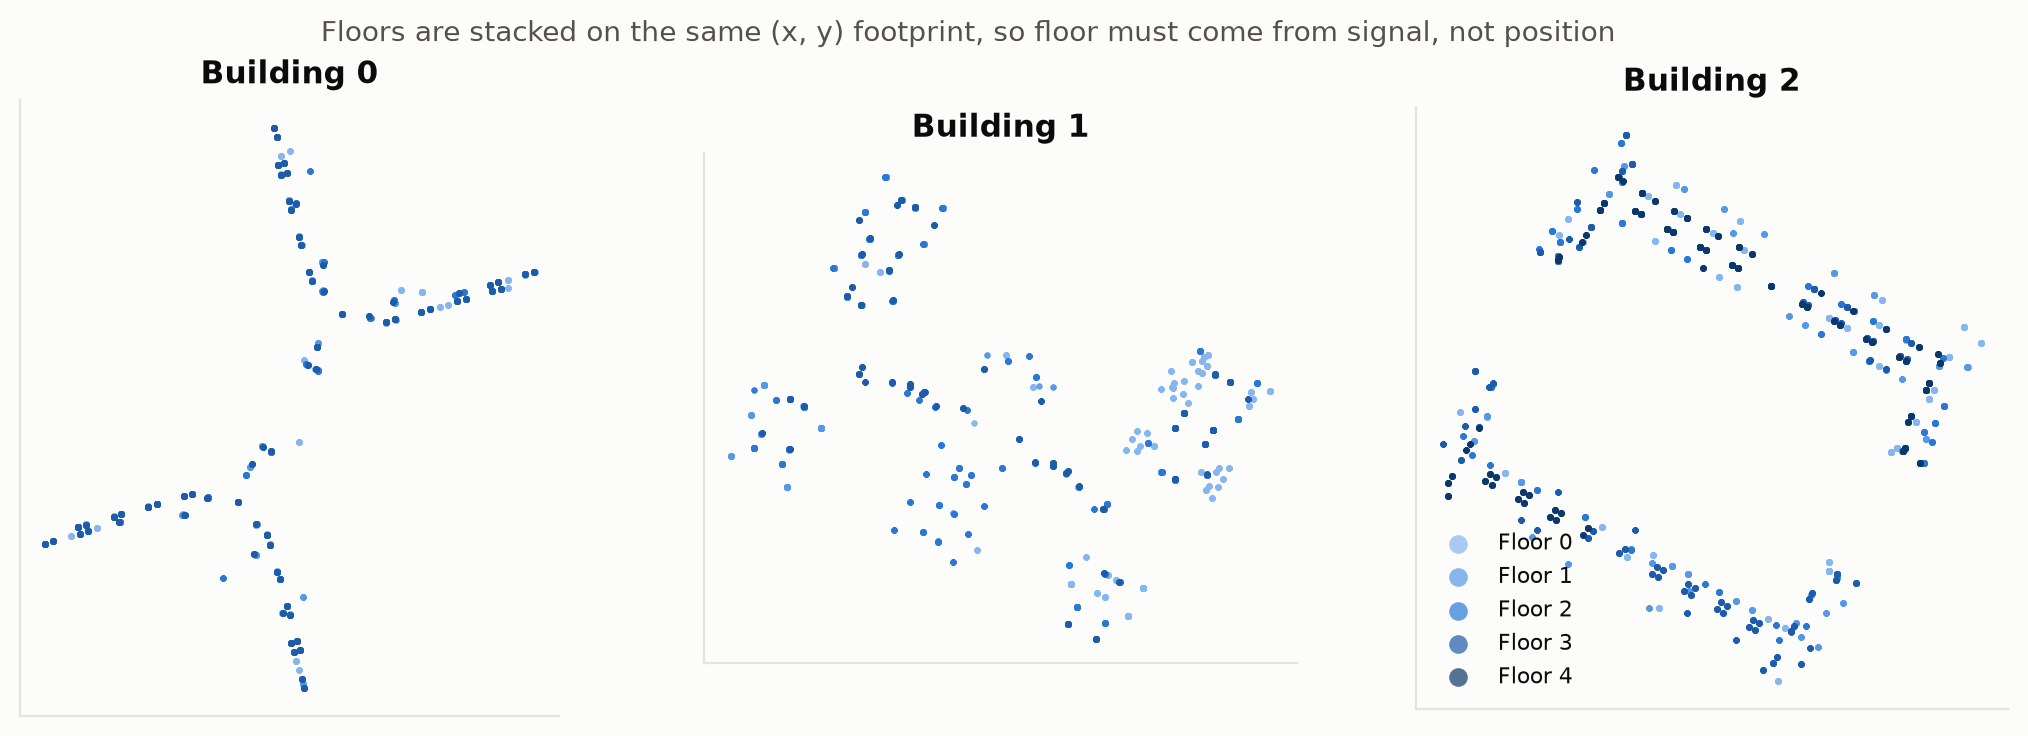
\includegraphics[width=\columnwidth]{eda_floors_per_building}
\caption{Training positions coloured by floor. Floors are stacked on the same $(x,y)$ footprint.}
\label{fig:floors}
\end{figure}

\textbf{Class balance and shift.} Training is fairly balanced over the 13 building--floor classes.
The test set is skewed: 48\% of test scans are in building 0, compared with 27\% in training (Fig.~\ref{fig:balance}).
Test phone proportions also differ (Fig.~\ref{fig:phones}), and 64\% of test scans come from phones
never seen in training. This makes the test set a realistic \emph{new users, new devices, later date} evaluation.

\begin{figure}[t]
\centering
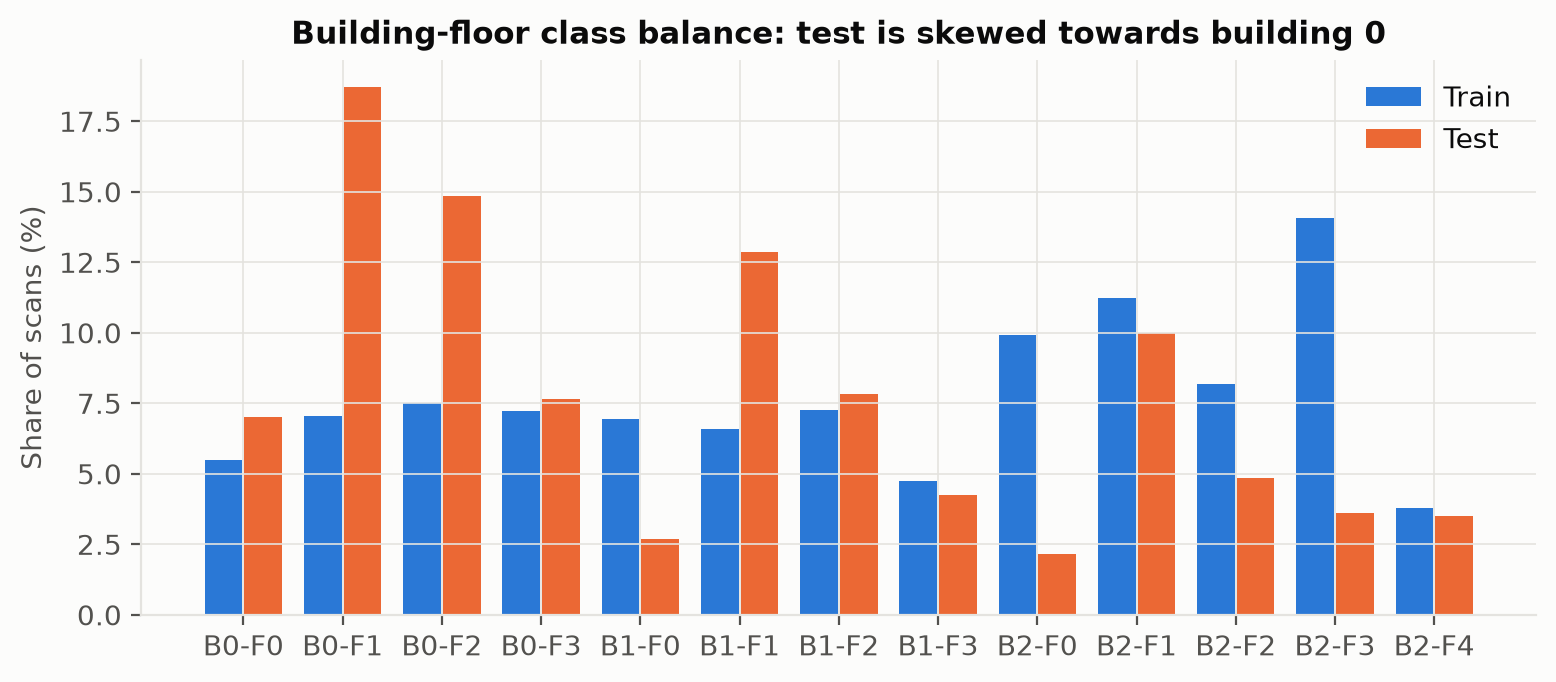
\includegraphics[width=\columnwidth]{eda_class_balance}
\caption{Share of scans per building--floor in train and test.}
\label{fig:balance}
\end{figure}

\begin{figure}[t]
\centering
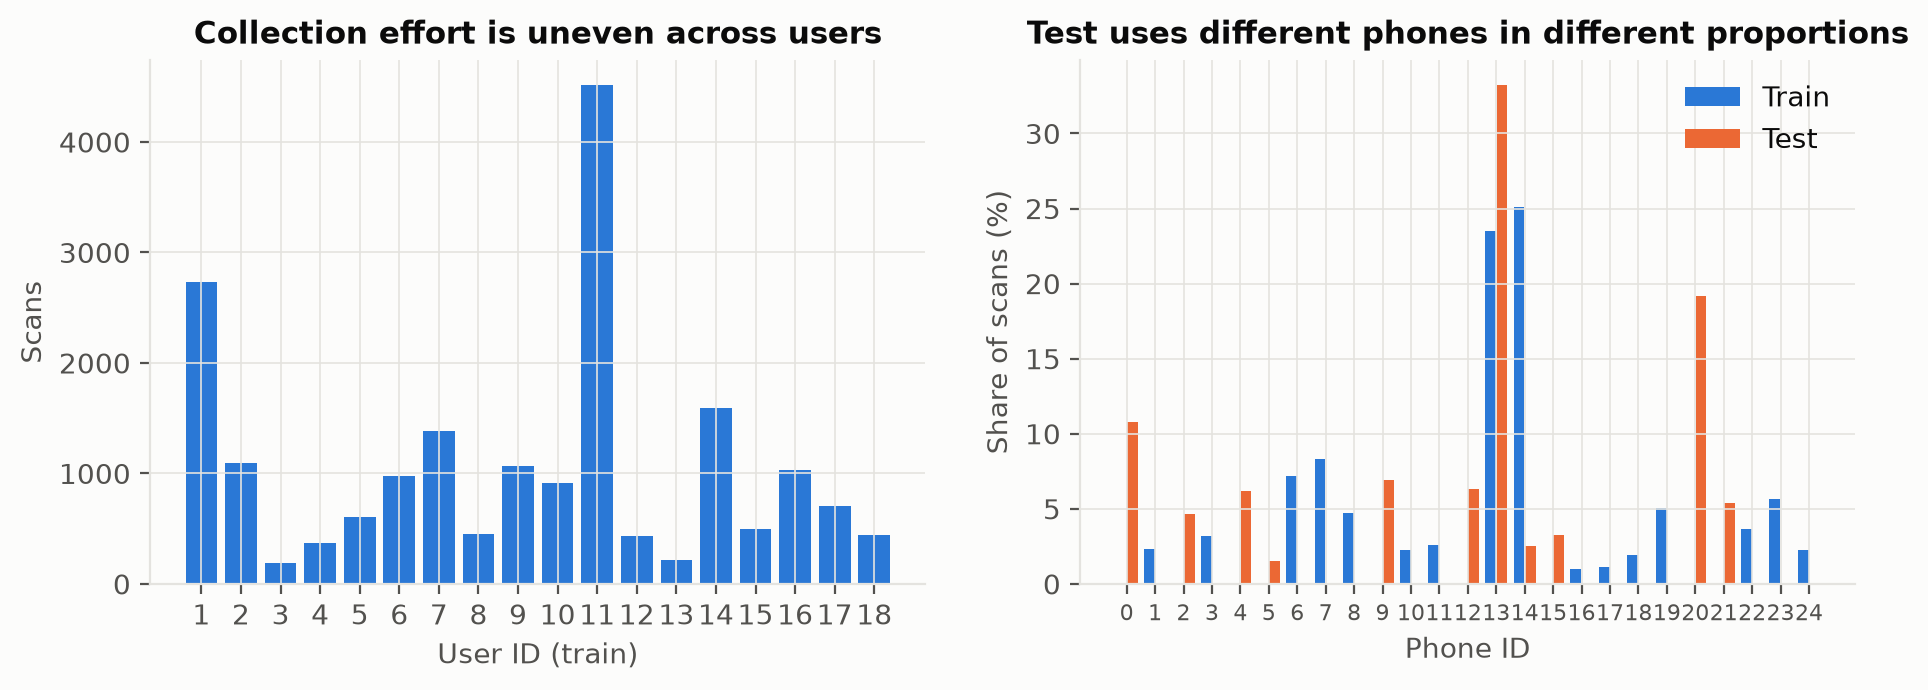
\includegraphics[width=\columnwidth]{eda_users_phones}
\caption{Scans per user (train) and per phone (train vs.\ test).}
\label{fig:phones}
\end{figure}

\textbf{Data quality.} 492 training scans contain readings above $-30$\,dBm, which is implausibly strong
for indoor Wi-Fi. 430 of them come from user~6 with phone~19 (Fig.~\ref{fig:suspicious}). We keep them by
default and test the effect of removing them in Section~\ref{sec:results}.

\begin{figure}[t]
\centering
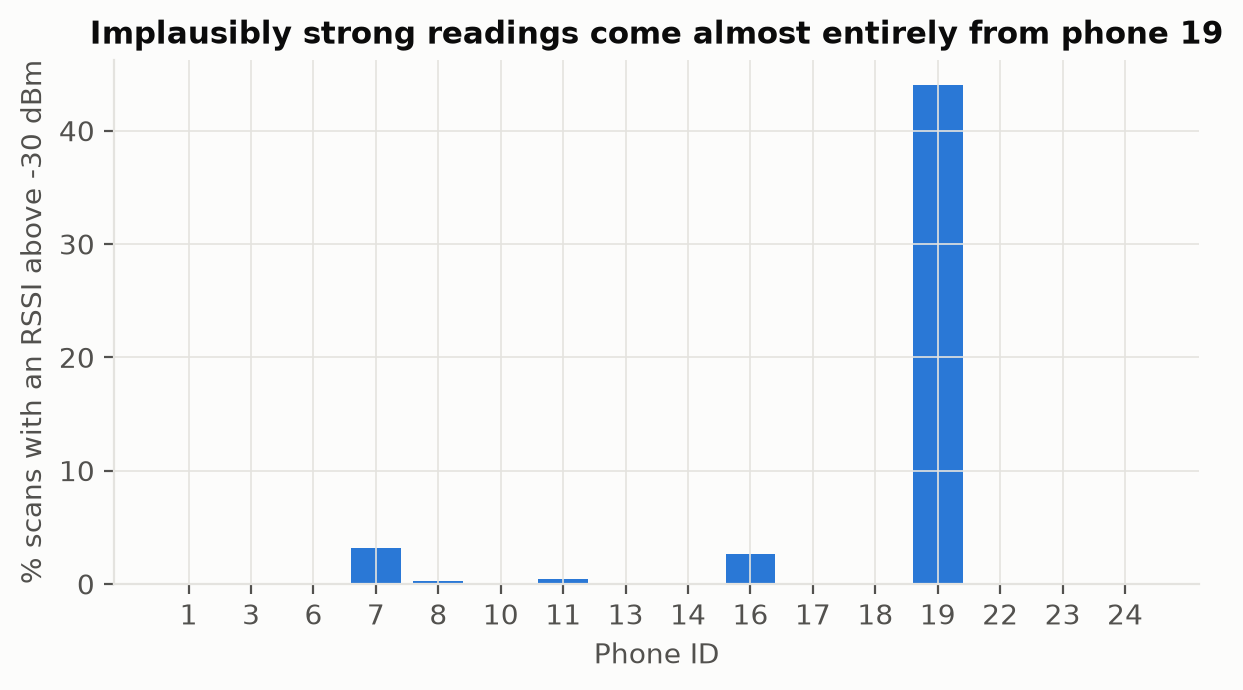
\includegraphics[width=0.85\columnwidth]{eda_suspicious_readings}
\caption{Share of scans with an RSSI above $-30$\,dBm, by phone.}
\label{fig:suspicious}
\end{figure}

\textbf{PCA.} With the missing values handled, the first two principal components already separate the three
buildings (Fig.~\ref{fig:pca}), but 50 components explain only 84\% of the variance. The useful
information is spread over many APs.

\begin{figure}[t]
\centering
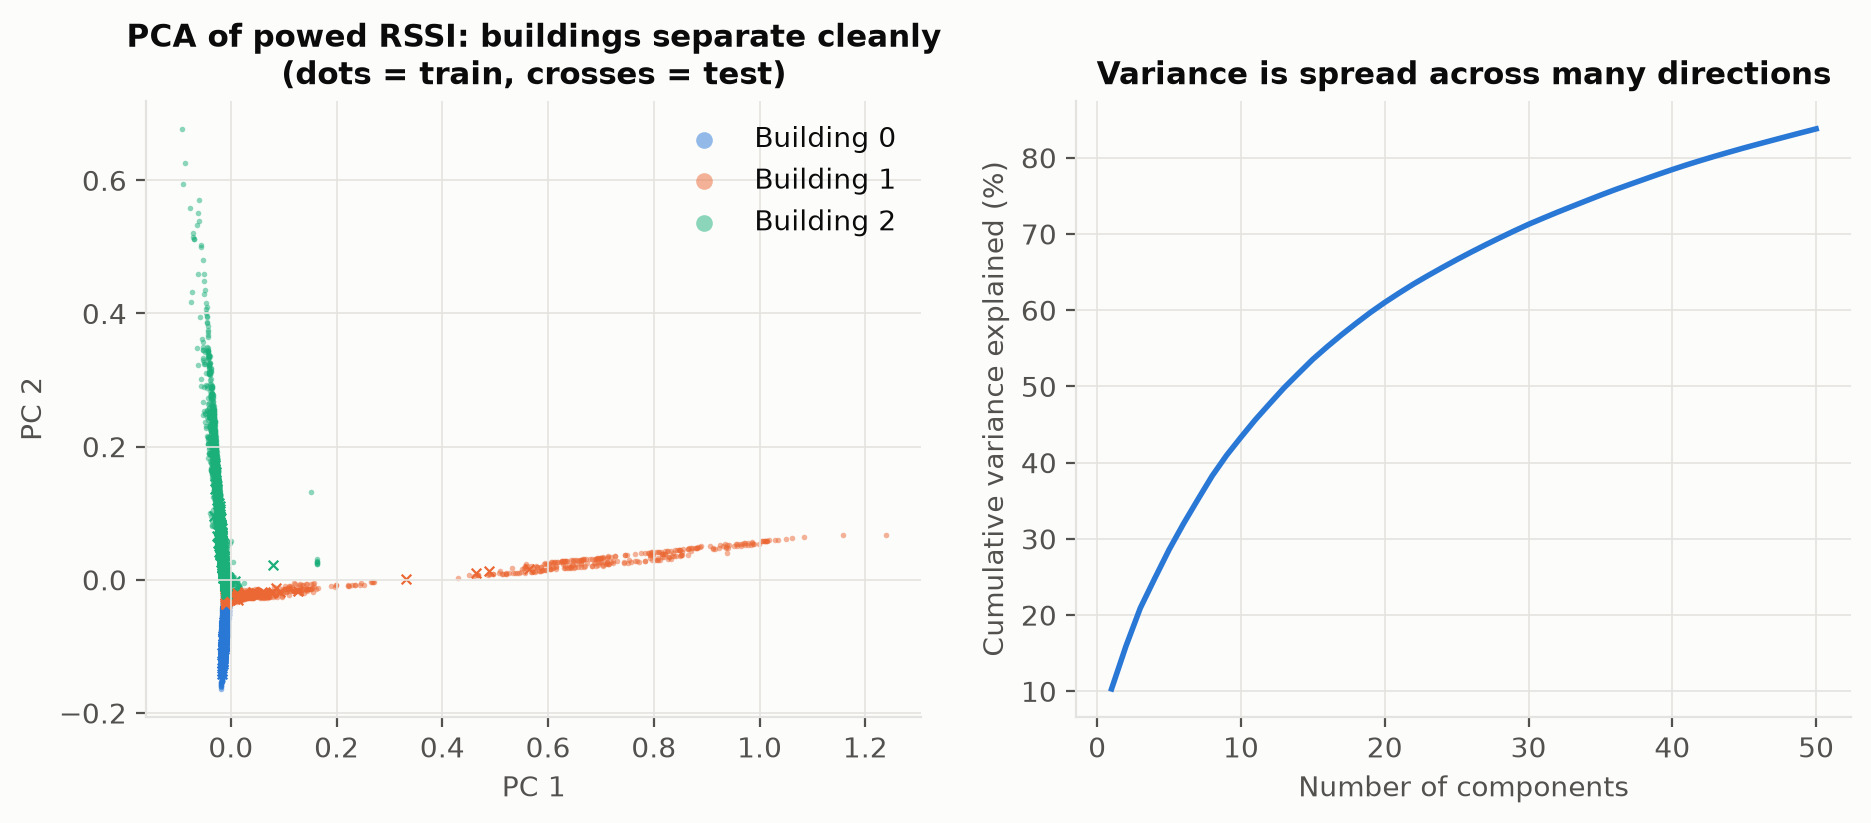
\includegraphics[width=\columnwidth]{eda_pca}
\caption{PCA of the RSSI matrix. Buildings separate; variance is spread across many directions.}
\label{fig:pca}
\end{figure}

\section{Methodology}
\subsection{Problem formulation}
Let $\mathbf{x}\in\mathbb{R}^{520}$ be a scan. We learn $f_b(\mathbf{x})\in\{0,1,2\}$,
$f_f(\mathbf{x})\in\{0,\dots,4\}$ and $f_p(\mathbf{x})\in\mathbb{R}^2$. Following the IPIN
competition~\cite{torres2017ipin}, the combined score of one prediction is
\begin{equation}
s = \lVert \mathbf{p}-\hat{\mathbf{p}}\rVert_2 + 50\cdot[b\neq\hat b] + 4\cdot[f\neq\hat f],
\label{eq:ipin}
\end{equation}
so a wrong building costs as much as 50\,m of error and a wrong floor costs 4\,m.

\subsection{Feature engineering}
\textbf{Missing signals.} ``Not detected'' means the signal is below the phone's sensitivity, so it is
\emph{missing not at random}: its absence tells us the AP is far away. Used as a number, $+100$\,dBm would look
like the strongest possible signal. We replace it with $m=\min(\text{observed})-1=-105$\,dBm, computed on training
data only. APs never heard in training are dropped, which leaves 465 features.

\textbf{Variants compared.} (a) \emph{raw}: dBm with $-105$ for not detected; (b) \emph{positive}: $x-m$, so not
detected is 0; (c) \emph{powed}: $\big((x-m)/(x_{\max}-m)\big)^{e}$, which compresses weak readings~\cite{torres2015distance};
(d) raw plus one binary heard/not-heard flag per AP; (e) (d) plus per-scan summaries (number of APs heard, strongest,
mean and standard deviation of RSSI, and the IDs of the three strongest APs). The variant for each model is chosen by
cross-validation.

\subsection{Models}
\textbf{Centroid baseline.} Predicts the most common building and floor and the mean position. It gives a floor against which to measure the other models.

\textbf{Linear and logistic regression.} Inputs are standardised with training statistics. Logistic
regression (softmax, cross-entropy, L2, $C=1$) predicts building and floor. Ordinary least-squares linear
regression predicts $x$ and $y$.

\textbf{$k$-NN}~\cite{cover1967nn}. The classic fingerprinting method: find the $k$ training scans
nearest in Euclidean distance. Building and floor come from a distance-weighted vote, and the position is the
distance-weighted mean of the neighbours' positions.

\textbf{Random Forest}~\cite{breiman2001rf}. An ensemble of CART trees. Each tree is grown on a bootstrap
sample, and each split considers a random subset of \texttt{max\_features} APs. Splits minimise Gini impurity
$G=1-\sum_k p_k^2$ for classification and variance for regression. For $B$ trees with variance $\sigma^2$ and
pairwise correlation $\rho$, the variance of their average is
\begin{equation}
\mathrm{Var}\Big(\tfrac{1}{B}\textstyle\sum_b T_b\Big)=\rho\sigma^2+\tfrac{1-\rho}{B}\sigma^2,
\end{equation}
so bagging removes the second term as $B$ grows and random feature selection lowers $\rho$.
Because a tree only compares a feature with a threshold, any order-preserving transform of the input gives the same tree.
A regression leaf predicts the mean of real training positions, so predictions never leave the surveyed area.

\textbf{Plain vs.\ per-building (hierarchical).} The \emph{plain} variant trains three independent forests on all
scans, as in the project brief. The \emph{per-building} variant predicts the building first, then sends the scan to a floor
forest and a position forest trained only on that building's scans. This turns one global problem into three
smaller, more homogeneous ones, at the risk that a wrong building prediction cascades to the floor and position.

\subsection{Validation protocol}
Consecutive scans by the same user at the same spot are near-duplicates, so a random split would leak them. We use
\textbf{5-fold GroupKFold with USERID as the group}: no user appears in both the training and validation parts of a fold. Feature
variants, $k$ and \texttt{max\_features} are all selected by the mean CV IPIN score. Imputation and scaling are
re-fitted inside every fold. The official validation file is used \textbf{once}, as the test set, after all
choices are fixed.

\section{Results}
\label{sec:results}
\subsection{Feature comparison}
Table~\ref{tab:ablation} compares the feature variants. The \emph{raw} and \emph{positive} variants give identical results for both
models, as theory predicts: the shift is order-preserving (trees) and cancels in Euclidean distances ($k$-NN).
None of the richer variants improved the CV score, so the simplest representation (raw dBm with $-105$ for not
detected) is used for every model. Powed features helped $k$-NN on the test set (IPIN 8.58 vs.\ 9.22) but hurt it
in CV (17.60 vs.\ 14.46). Because test scores must not drive selection, we did not adopt them.

\begin{table}[t]
\centering
\caption{Feature comparison. CV $=$ 5-fold GroupKFold by user on the training set (used to choose); test shown for reference only.}
\label{tab:ablation}
\resizebox{\columnwidth}{!}{%
\begin{tabular}{lcccc}
\toprule
Features & CV IPIN & Test IPIN & Test B+F \% & Test err. (m) \\
\midrule
\multicolumn{5}{l}{\emph{Random Forest (per-building)}} \\
raw dBm, not-heard = -105 & 15.23 & 9.70 & 91.18 & 9.31 \\
positive (shifted so not-heard = 0) & 15.23 & 9.70 & 91.18 & 9.31 \\
powed (compress weak signals) & 15.71 & 9.88 & 91.09 & 9.44 \\
raw + heard/not-heard flags & 15.55 & 10.28 & 90.28 & 9.80 \\
raw + flags + scan summary & 15.82 & 9.86 & 91.00 & 9.50 \\
\midrule
\multicolumn{5}{l}{\emph{k-NN (k=5)}} \\
raw dBm, not-heard = -105 & 14.46 & 9.22 & 90.10 & 8.69 \\
positive (shifted so not-heard = 0) & 14.46 & 9.22 & 90.10 & 8.69 \\
powed (compress weak signals) & 17.60 & 8.58 & 93.43 & 8.19 \\
raw + heard/not-heard flags & 14.54 & 9.20 & 90.01 & 8.66 \\
\bottomrule
\end{tabular}}
\end{table}


\subsection{Tuning}
Table~\ref{tab:tuning} shows the CV search. For $k$-NN, $k=5$ is best: $k=1$ is noisy and $k=11$ over-smooths.
For the Random Forest, \texttt{max\_features}$=\sqrt{p}$ ($\approx$21 APs per split) beats 10\% and 30\%, because
more random, less correlated trees average better. The error drops quickly up to about 50 trees and is flat beyond 100
(Fig.~\ref{fig:tuning}), so 300 trees is safely on the plateau. In CV, $k$-NN scores slightly better than the forest
(IPIN 14.46 vs.\ 15.21; floor accuracy 74.1\% vs.\ 71.3\%), while the forest identifies the building more reliably (99.0\% vs.\ 96.7\%).

\begin{table}[t]
\centering
\caption{Hyper-parameter search with user-grouped 5-fold CV on the training set.}
\label{tab:tuning}
\resizebox{\columnwidth}{!}{%
\begin{tabular}{llccc}
\toprule
Model & Parameters & B+F \% & Mean err. (m) & IPIN \\
\midrule
k-NN & k=1 & 72.38 & 12.92 & 15.55 \\
k-NN & k=3 & 72.30 & 12.10 & 14.71 \\
k-NN & k=5 & 72.29 & 11.78 & 14.46 \\
k-NN & k=7 & 72.26 & 11.80 & 14.73 \\
k-NN & k=11 & 72.06 & 11.93 & 15.05 \\
Random Forest & max\_features=sqrt, n\_estimators=300 & 70.90 & 13.55 & 15.21 \\
Random Forest & max\_features=0.1, n\_estimators=300 & 71.56 & 14.38 & 16.08 \\
Random Forest & max\_features=0.3, n\_estimators=300 & 70.93 & 15.57 & 17.45 \\
\bottomrule
\end{tabular}}
\end{table}


\begin{figure}[t]
\centering
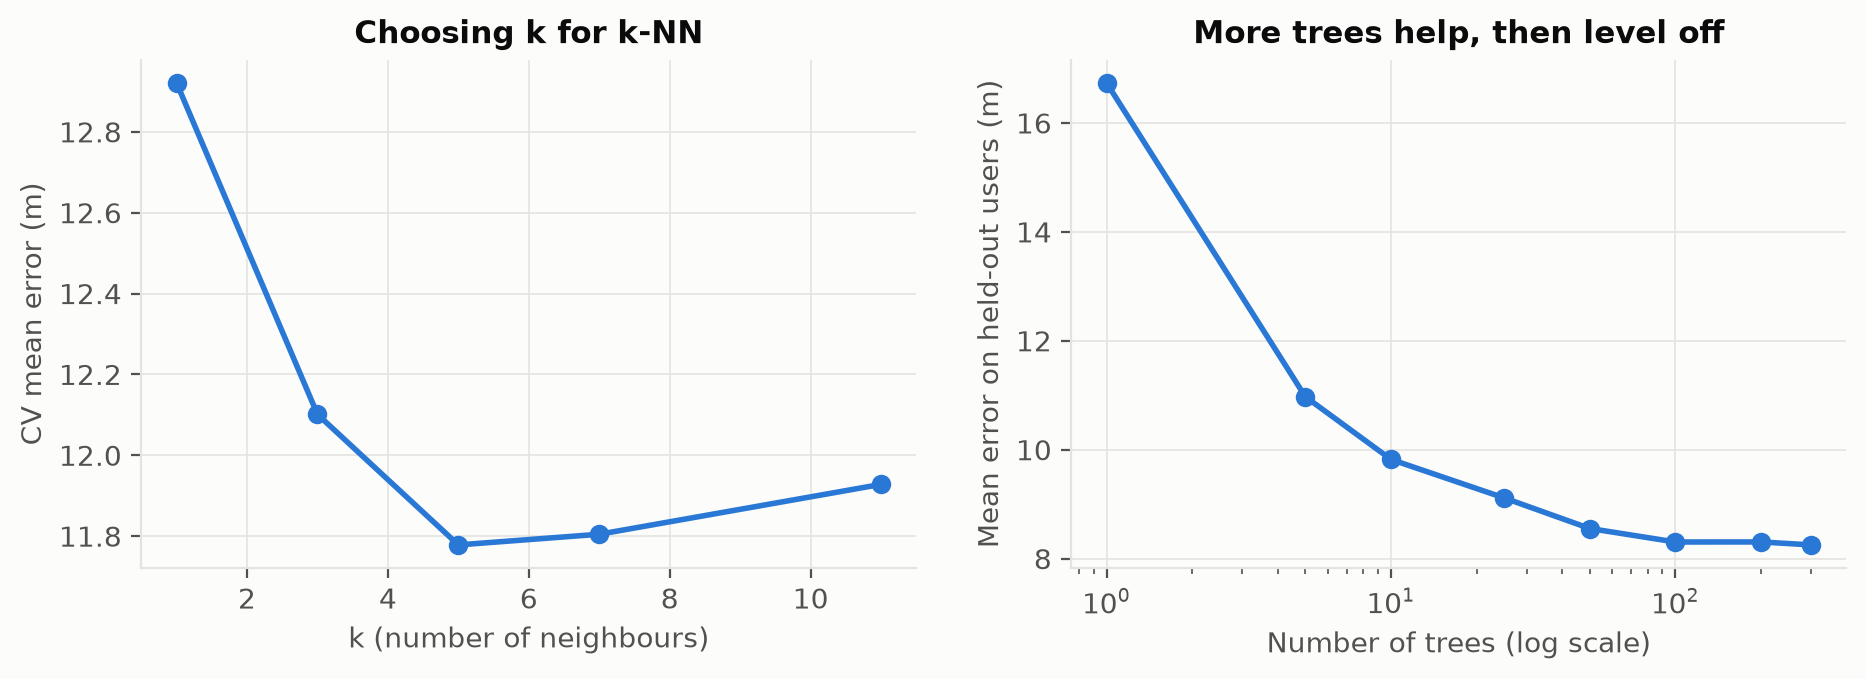
\includegraphics[width=\columnwidth]{tuning_curves}
\caption{Left: CV error vs.\ $k$. Right: error on held-out users vs.\ number of trees.}
\label{fig:tuning}
\end{figure}

\subsection{Test-set comparison}
Table~\ref{tab:main} and Fig.~\ref{fig:comparison} report the single evaluation on the official test set.
All learned models identify the building almost perfectly. Logistic regression even gets 100\%, because buildings
use disjoint APs. On floor, the per-building Random Forest is best (91.3\%), ahead of the plain forest (90.9\%),
$k$-NN (90.1\%) and logistic regression (88.7\%). For position, linear regression is unusable (52.0\,m), while
$k$-NN (8.69\,m) and the per-building forest (9.37\,m) are close. The per-building design lowers the forest's error
from 10.22\,m to 9.37\,m and its 95th-percentile error from 27.4\,m to 23.3\,m, the lowest tail of all models
(Fig.~\ref{fig:cdf}). For reference, the dataset paper's $k$-NN baseline reported 89.9\% floor accuracy and 7.9\,m mean
error~\cite{torres2014uji}.

\begin{table*}[t]
\centering
\caption{Test-set results (official UJIIndoorLoc validation file, 1{,}111 scans). Accuracies in \%, errors in metres.
IPIN score $=$ 2-D error $+\,50\times$ building miss $+\,4\times$ floor miss.}
\label{tab:main}
\begin{tabular}{lccccccc}
\toprule
Model & Building & Floor & Bldg+Floor & Mean err. & Median & P75 & IPIN score \\
\midrule
Centroid (guess the average) & 24.12 & 15.48 & 3.60 & 142.75 & 167.37 & 193.37 & 184.07 \\
Linear + Logistic Regression & 100.00 & 88.66 & 88.66 & 51.99 & 37.53 & 72.25 & 52.45 \\
k-NN & 99.73 & 90.10 & 90.10 & \textbf{8.69} & 5.35 & 10.31 & 9.22 \\
Random Forest & 99.82 & 90.91 & 90.82 & 10.22 & 7.63 & 13.35 & 10.68 \\
Random Forest (per-building) & 99.82 & 91.27 & \textbf{91.18} & 9.37 & 7.07 & 12.19 & 9.81 \\
\bottomrule
\end{tabular}
\end{table*}


\begin{figure}[t]
\centering
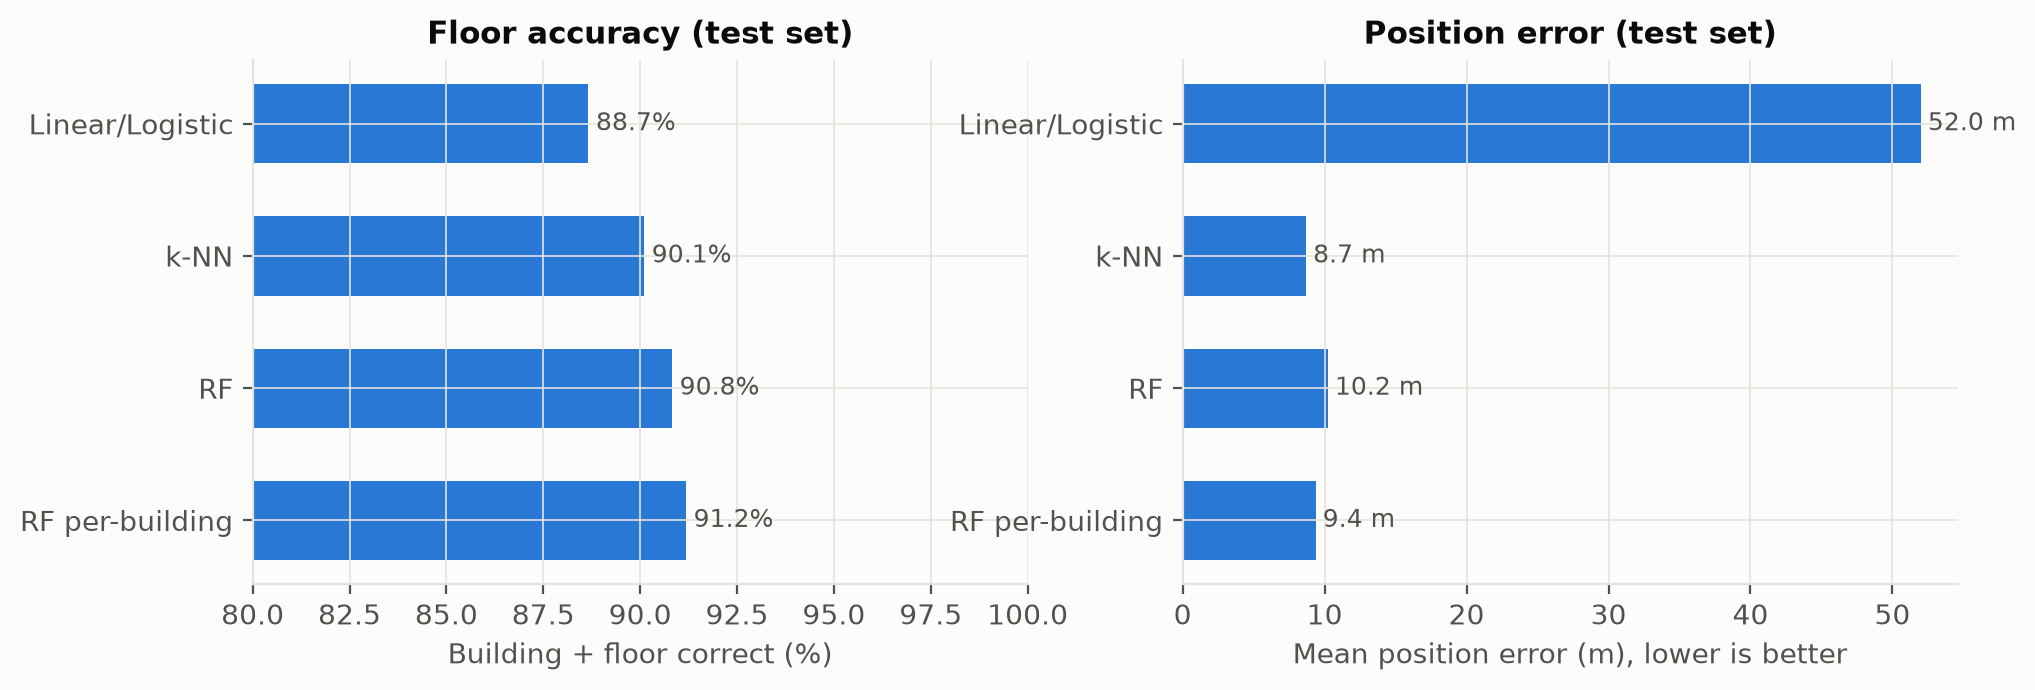
\includegraphics[width=\columnwidth]{model_comparison}
\caption{Floor accuracy and mean position error on the test set (centroid baseline omitted: 3.6\%, 142.8\,m).}
\label{fig:comparison}
\end{figure}

\begin{figure}[t]
\centering
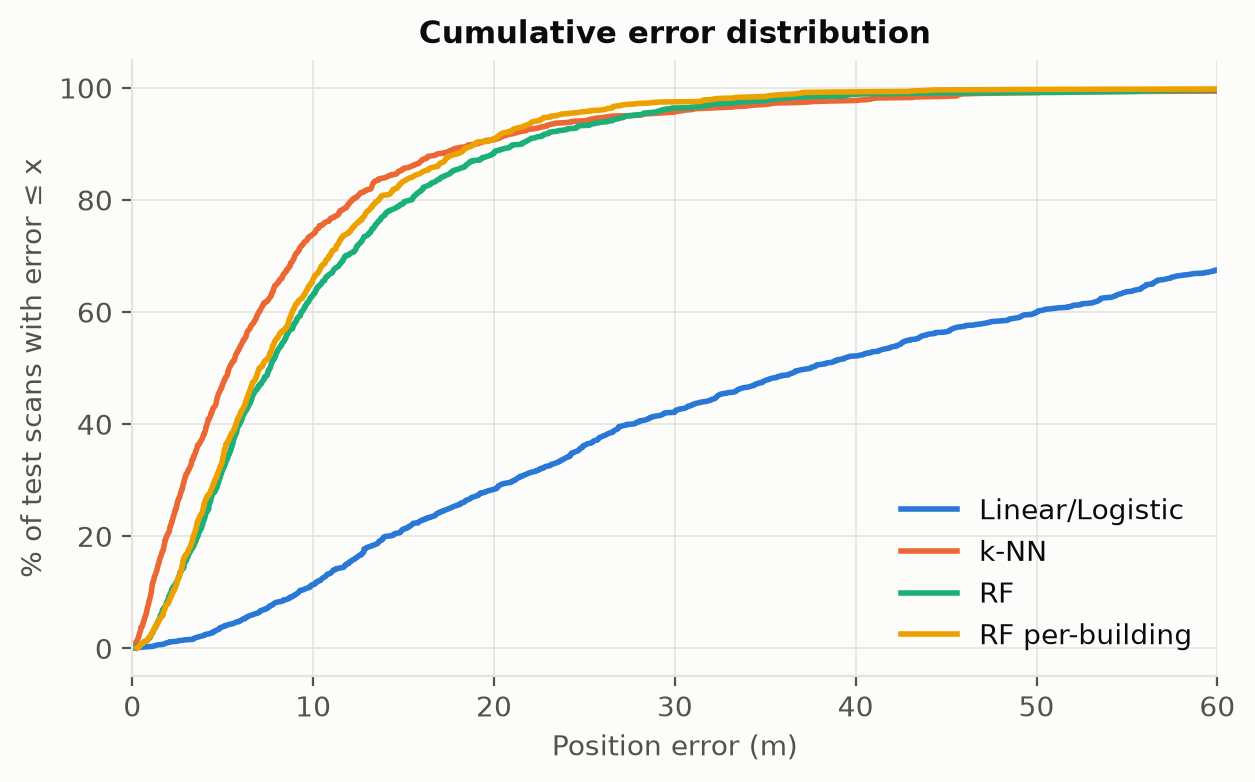
\includegraphics[width=0.85\columnwidth]{error_cdf}
\caption{Cumulative distribution of position error.}
\label{fig:cdf}
\end{figure}

\subsection{Error analysis}
\textbf{Hierarchical breakdown} (Table~\ref{tab:breakdown}). For the per-building forest, only 2 of 1{,}111 scans
have the wrong building, but they are far off (107\,m). The 96 scans with the right building but wrong floor average 15.7\,m,
almost twice the 8.6\,m of fully correct scans. Most of the total error (83\%) still comes from correct-floor scans, so
improving within-floor positioning matters as much as floor classification.

\begin{table}[t]
\centering
\caption{Error split by whether building and floor were right, Random Forest (per-building) (test set).}
\label{tab:breakdown}
\resizebox{\columnwidth}{!}{%
\begin{tabular}{lcccc}
\toprule
Case & $n$ & Mean (m) & Median (m) & Share of total error \% \\
\midrule
building ok, floor ok & 1013 & 8.57 & 6.65 & 83.4 \\
building ok, floor wrong & 96 & 15.73 & 12.55 & 14.5 \\
building wrong & 2 & 107.25 & 107.25 & 2.1 \\
\bottomrule
\end{tabular}}
\end{table}


\textbf{Floors} (Fig.~\ref{fig:confusion}). Building~0 is easy (97.6\%). Building~1 is the weak spot (79.8\%):
43 of its 143 floor-1 test scans are predicted as floor~2. Errors are almost always between \emph{adjacent} floors, as
expected when signals leak through one ceiling.

\begin{figure*}[t]
\centering
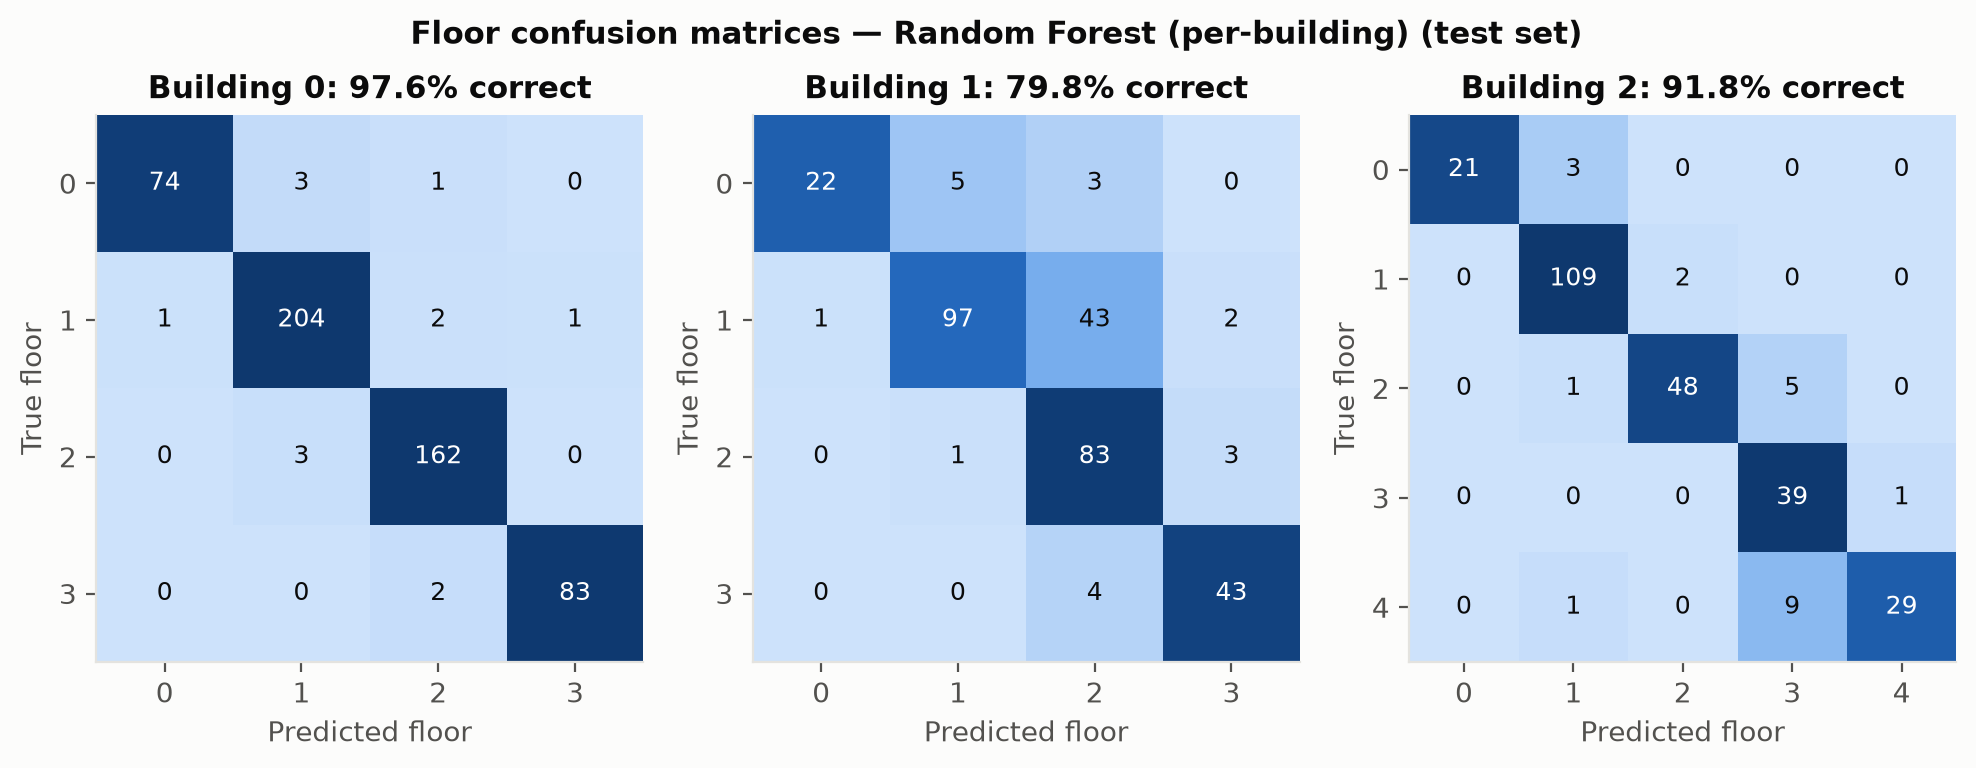
\includegraphics[width=0.85\textwidth]{confusion_floor_rf}
\caption{Floor confusion matrices of the per-building Random Forest on the test set.}
\label{fig:confusion}
\end{figure*}

\textbf{Spatial errors} (Fig.~\ref{fig:errmap}). Building~0 has the lowest error (6.5--7.5\,m per floor). The worst
building--floors are building~2 floor~2 (17.6\,m) and floor~4 (16.2\,m).

\begin{figure}[t]
\centering
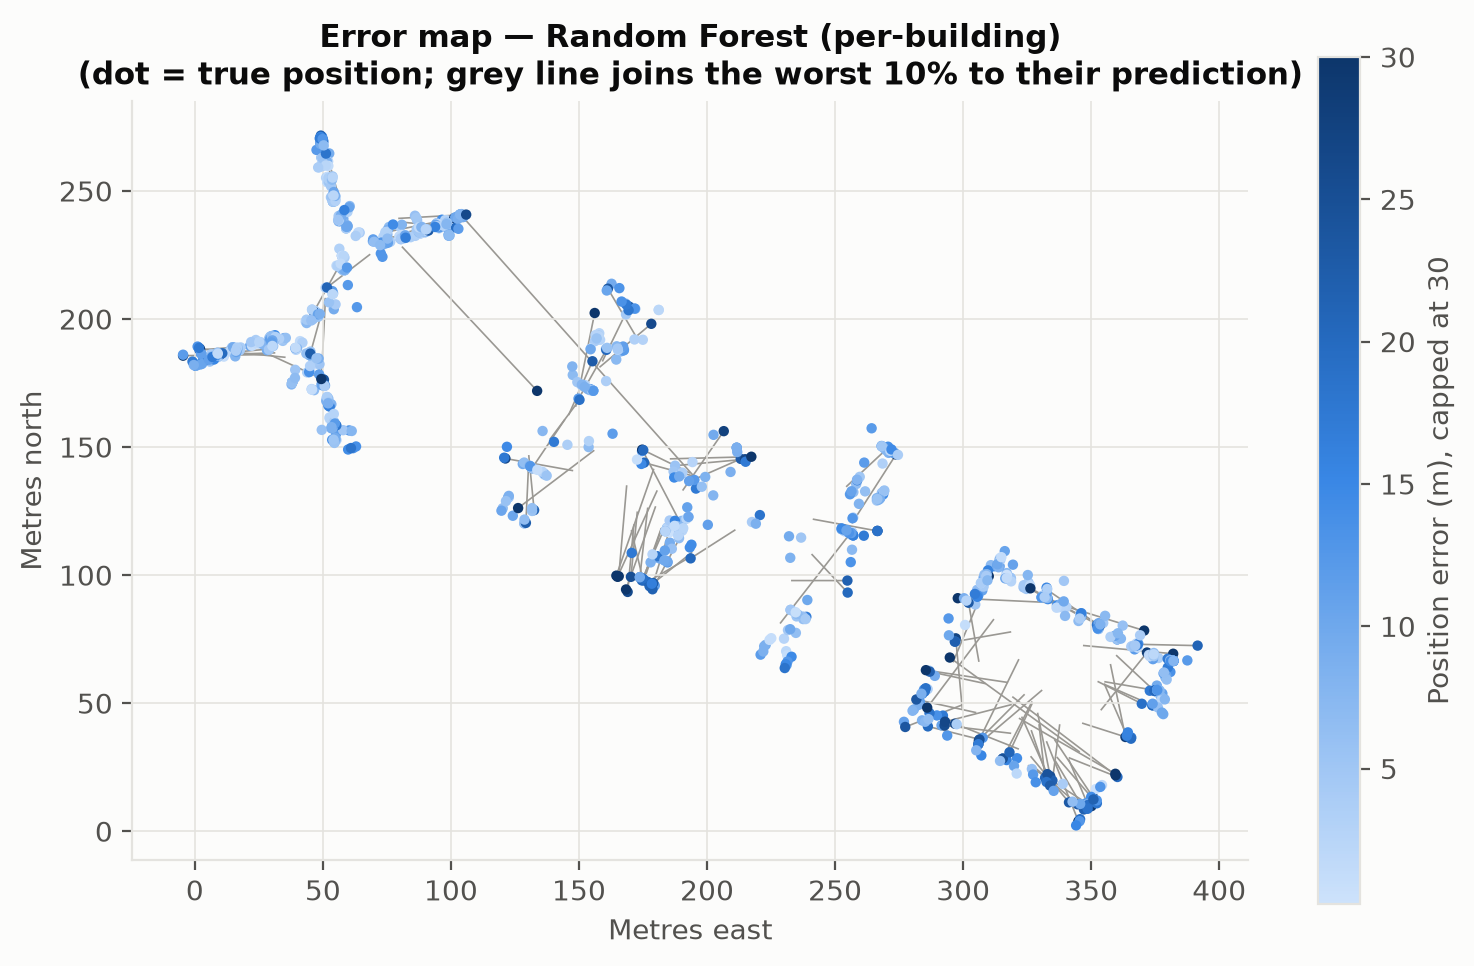
\includegraphics[width=\columnwidth]{error_map_rf}
\caption{Coordinate error map (per-building RF). Grey lines join the worst 10\% of predictions to the true position.}
\label{fig:errmap}
\end{figure}

\textbf{Coverage and devices} (Figs.~\ref{fig:aps},~\ref{fig:phone}). Scans that hear 5 or fewer APs have the largest error (27.9\,m, $n=18$).
Error also rises for scans that hear more than 25 APs: 105 of these 141 scans come from phone~20, a phone absent from training that
hears more APs per scan than any other test phone (25 on average) and is itself one of the least accurate phones (13.2\,m). Across test phones, mean error ranges from 6.2\,m (phone~9)
to 16.3\,m (phone~14), so device heterogeneity is a real source of error.

\begin{figure}[t]
\centering
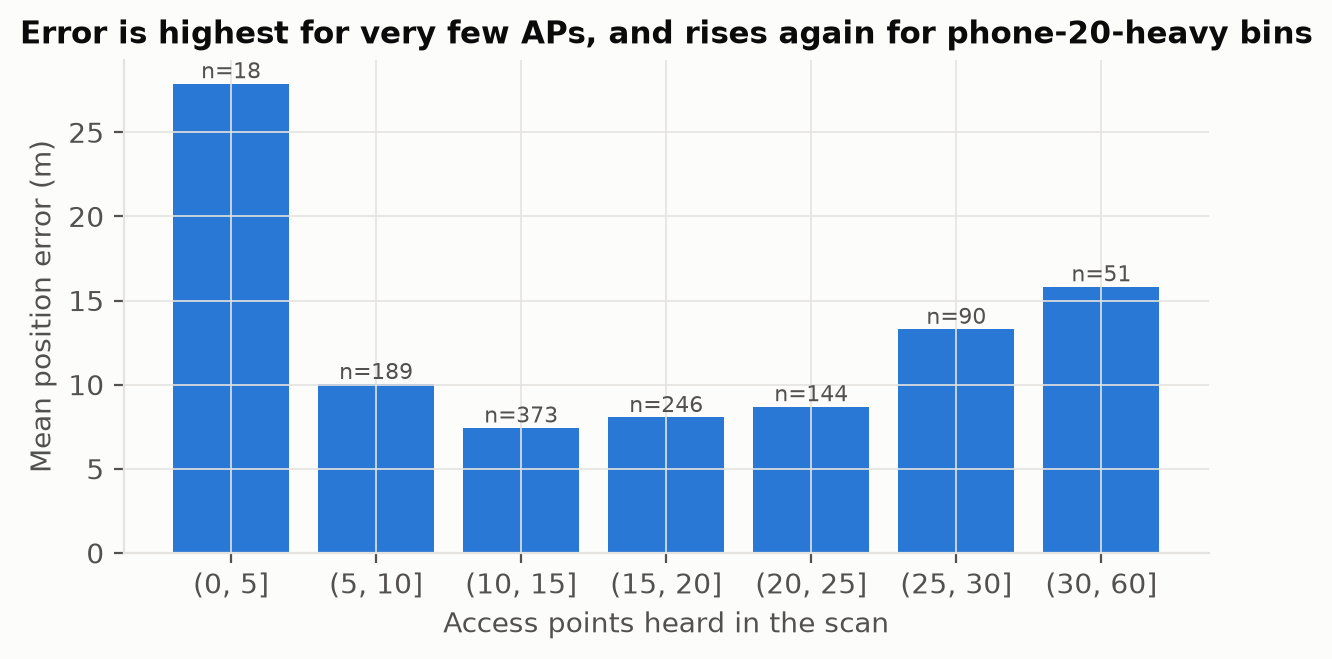
\includegraphics[width=0.85\columnwidth]{error_vs_aps_heard}
\caption{Mean error by number of APs heard in the test scan.}
\label{fig:aps}
\end{figure}

\begin{figure}[t]
\centering
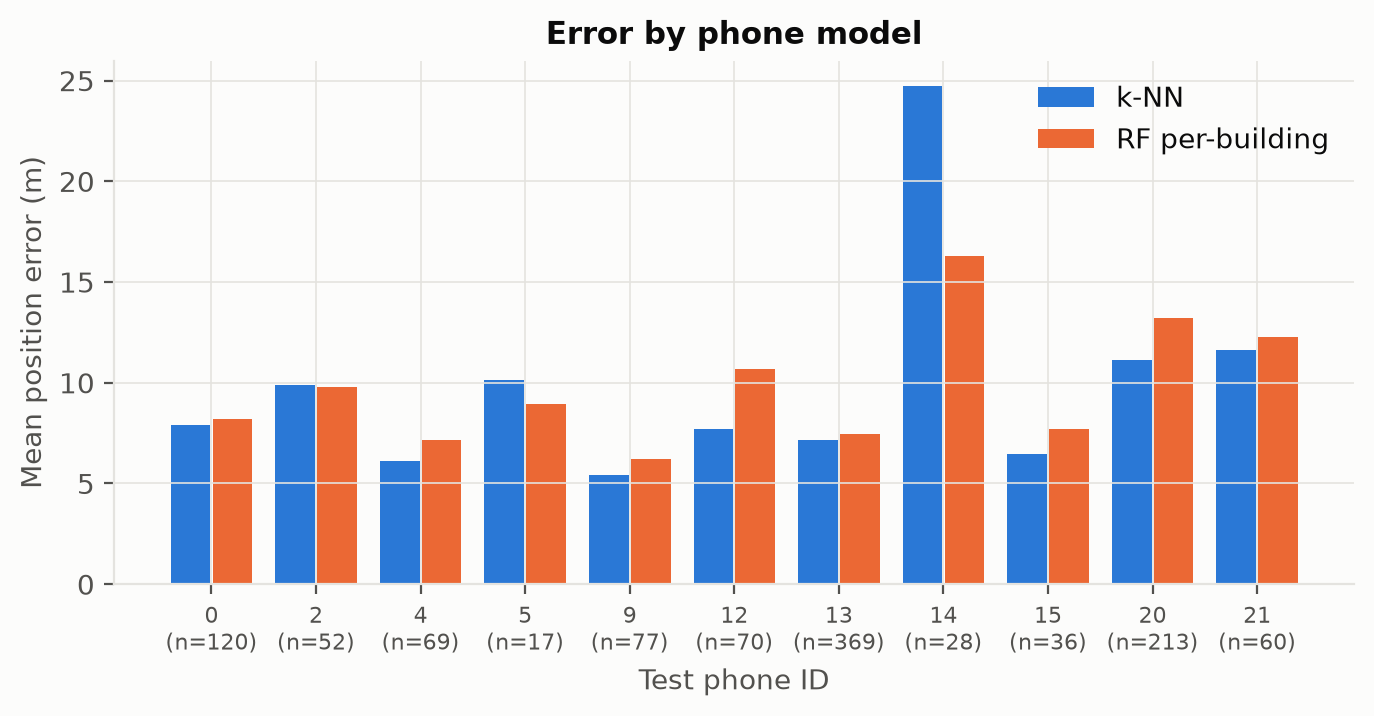
\includegraphics[width=\columnwidth]{per_phone_error}
\caption{Mean position error per test phone.}
\label{fig:phone}
\end{figure}

\textbf{Outliers and importance.} Removing the 492 scans with readings above $-30$\,dBm did not help
(9.46\,m vs.\ 9.37\,m), so the forest is already robust to them. Feature importance (Fig.~\ref{fig:importance}) shows that the
building classifier spreads its importance over many APs instead of relying on a single one.

\begin{figure}[t]
\centering
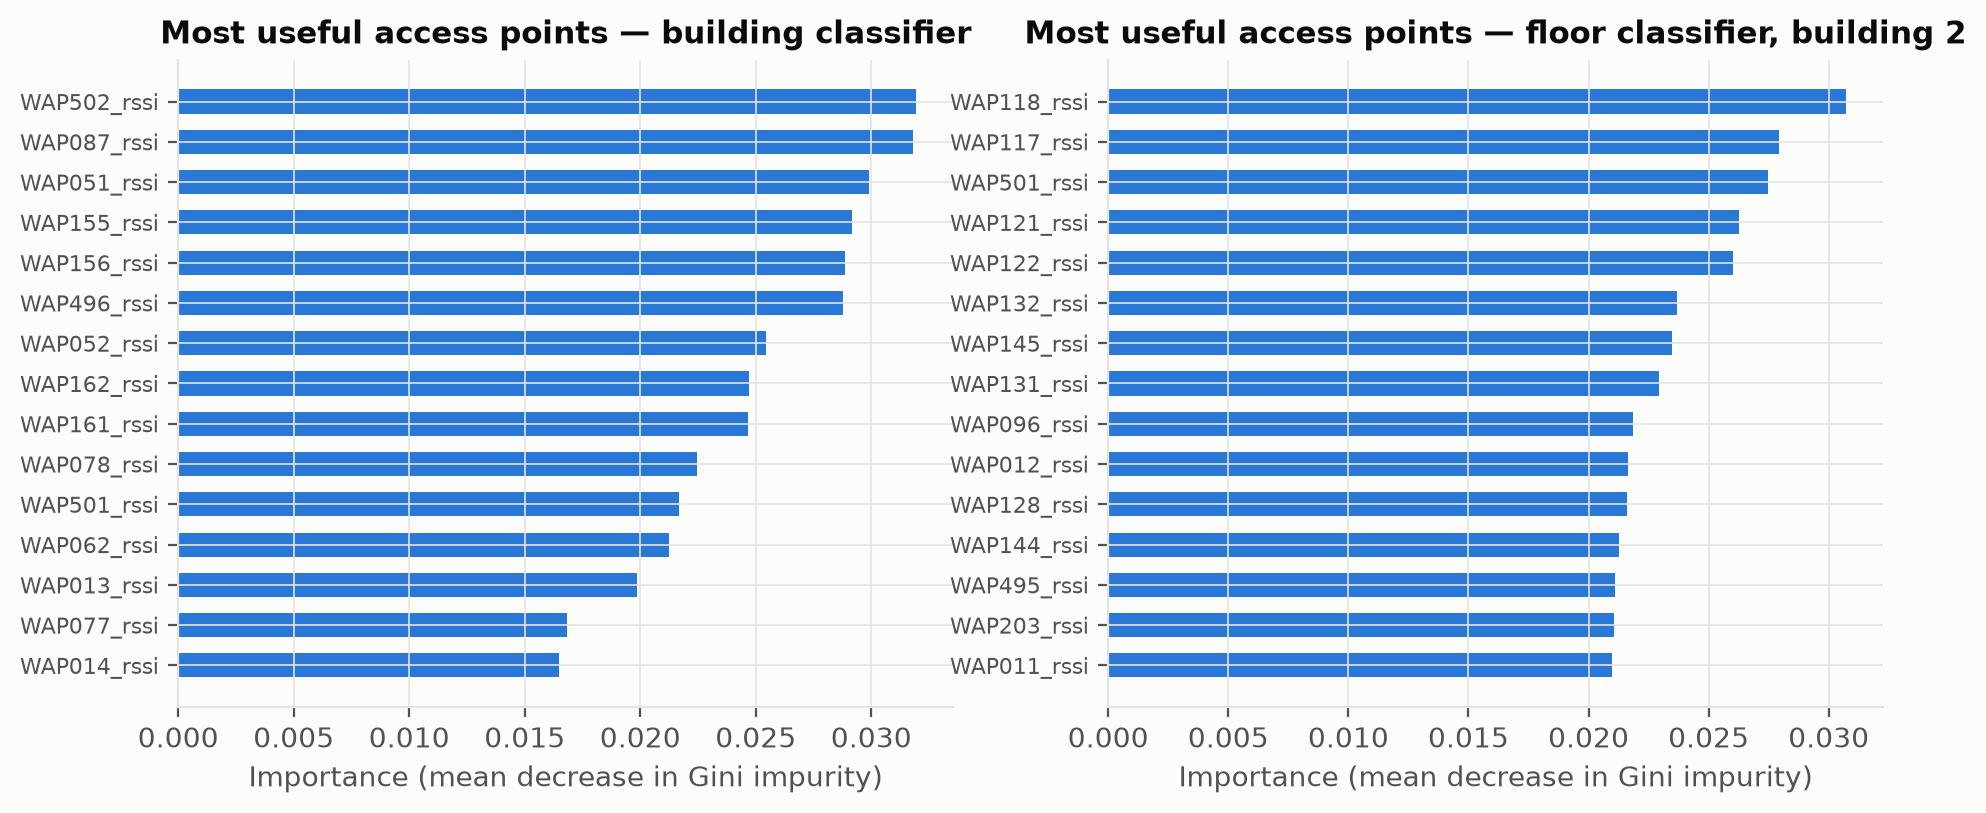
\includegraphics[width=\columnwidth]{feature_importance}
\caption{Top-15 APs by Gini importance for the building and building-2 floor classifiers.}
\label{fig:importance}
\end{figure}


\section{Discussion}
\textbf{Why linear models fail at position but not at building.} Building identity is almost a linear function of which
APs are heard, so a weighted sum separates it. Position is not: RSSI falls with the \emph{logarithm} of distance, walls cut it abruptly,
and the same AP is ``east of you'' in one corridor and ``west'' in another. A single hyperplane cannot represent this. Trees and $k$-NN
make local, piecewise decisions and therefore can.

\textbf{$k$-NN vs.\ Random Forest.} The two are close, and the ranking depends on the evaluation: $k$-NN is ahead in CV, and on
test it has the lower mean (8.69\,m) and median (5.36\,m) error, while the per-building forest has the best floor accuracy and the lightest error
tail on test. $k$-NN copies the positions of real neighbouring fingerprints, which works well when the radio map is dense. The forest
learns which APs matter. We keep the Random Forest as the main model because the brief asks for it and it is strongest on floor, the hardest
target on the test set, and we report $k$-NN alongside it.

\textbf{CV vs.\ test.} CV is much harsher than test (floor accuracy about 72\% vs.\ 91\%; mean error 12--14\,m vs.\ 9\,m). We ruled out
location coverage: 9.9\% of CV scans and 7.7\% of test scans are more than 5\,m from any training point. The likely cause is device novelty.
In training, 17 of 18 users carried their own phone, so almost every CV validation scan comes from an unseen device, whereas 35.7\% of test
scans come from phones seen in training. User-grouped CV is therefore a strict but honest selection criterion.

\textbf{The gap for Phase 2.} All our models treat building, floor and position as separate tasks. The per-building forest links
them only through a fixed cascade, and its two wrong-building scans are its worst errors. None of the models learns a representation of the 465 interacting APs that the three tasks could share.

\section{Conclusion and Phase 2 Plan}
We built a leakage-free machine learning pipeline for Wi-Fi indoor positioning on UJIIndoorLoc. The key data
decisions were to treat ``not detected'' as a very weak signal ($-105$\,dBm) fitted on training data only, and to validate by holding out
whole users. Simple raw features were as good as the engineered variants. A per-building Random Forest reaches 99.8\%
building accuracy, 91.3\% floor accuracy and 9.37\,m mean error on a test set collected months later with mostly unseen phones.
$k$-NN is a close second. Remaining errors come from adjacent-floor confusion (especially building~1), scans that hear very few APs, and device differences.

In Phase~2 we will train a \textbf{multitask MLP} with a shared trunk and three heads (building and floor softmax, coordinate
regression), optimised with $\mathcal{L}=\lambda_b\mathrm{CE}_b+\lambda_f\mathrm{CE}_f+\lambda_p\mathrm{MSE}_p$~\cite{caruana1997mtl},
regularised with dropout, weight decay and early stopping on the same user-grouped validation. We will compare it with these baselines on the
identical split and metrics, and run ablations (single-task vs.\ multitask, loss weights).

\section*{Team Contributions}
\begin{tabular}{@{}p{0.27\columnwidth}p{0.66\columnwidth}@{}}
Rishi Raj & Literature review, problem framing, evaluation metrics \\
Aditya Samadhiya & Data cleaning and exploratory data analysis \\
Yash Yadav & Feature engineering and feature comparison \\
Kaustubh Ranjan Mishra & Linear/logistic and $k$-NN models, cross-validation design \\
Yash Raj & Random Forest models, error analysis, repository and report \\
\end{tabular}

\section*{Reproducibility}
Code, figures and an executed notebook are in the project GitHub repository. Running
\texttt{python scripts/download\_data.py}, \texttt{run\_eda.py} and \texttt{run\_experiments.py} reproduces every number
(random seed 42).

\bibliographystyle{IEEEtran}
\bibliography{refs}

\end{document}
